
\paragraph{LDM Attempt 2}\mbox{}\\

\indent In this attempt instead of creating noise from $\sim\mathcal{N}(0,1)$, the noise was generated from $N(\mu, \sigma)$ where $\mu$ is the mean of the training data $z_{\mu}$ and $\sigma$ is the mean of $z_{\sigma}$ obtained from the training data set (25 samples).

\paragraph{Model configuration}\mbox{}\\
The configuration was the same as in Attempt 1. The only difference was in the noise generation approach.

\paragraph{Training}\mbox{}\\
\begin{figure}[H]
\minipage{0.49\textwidth}
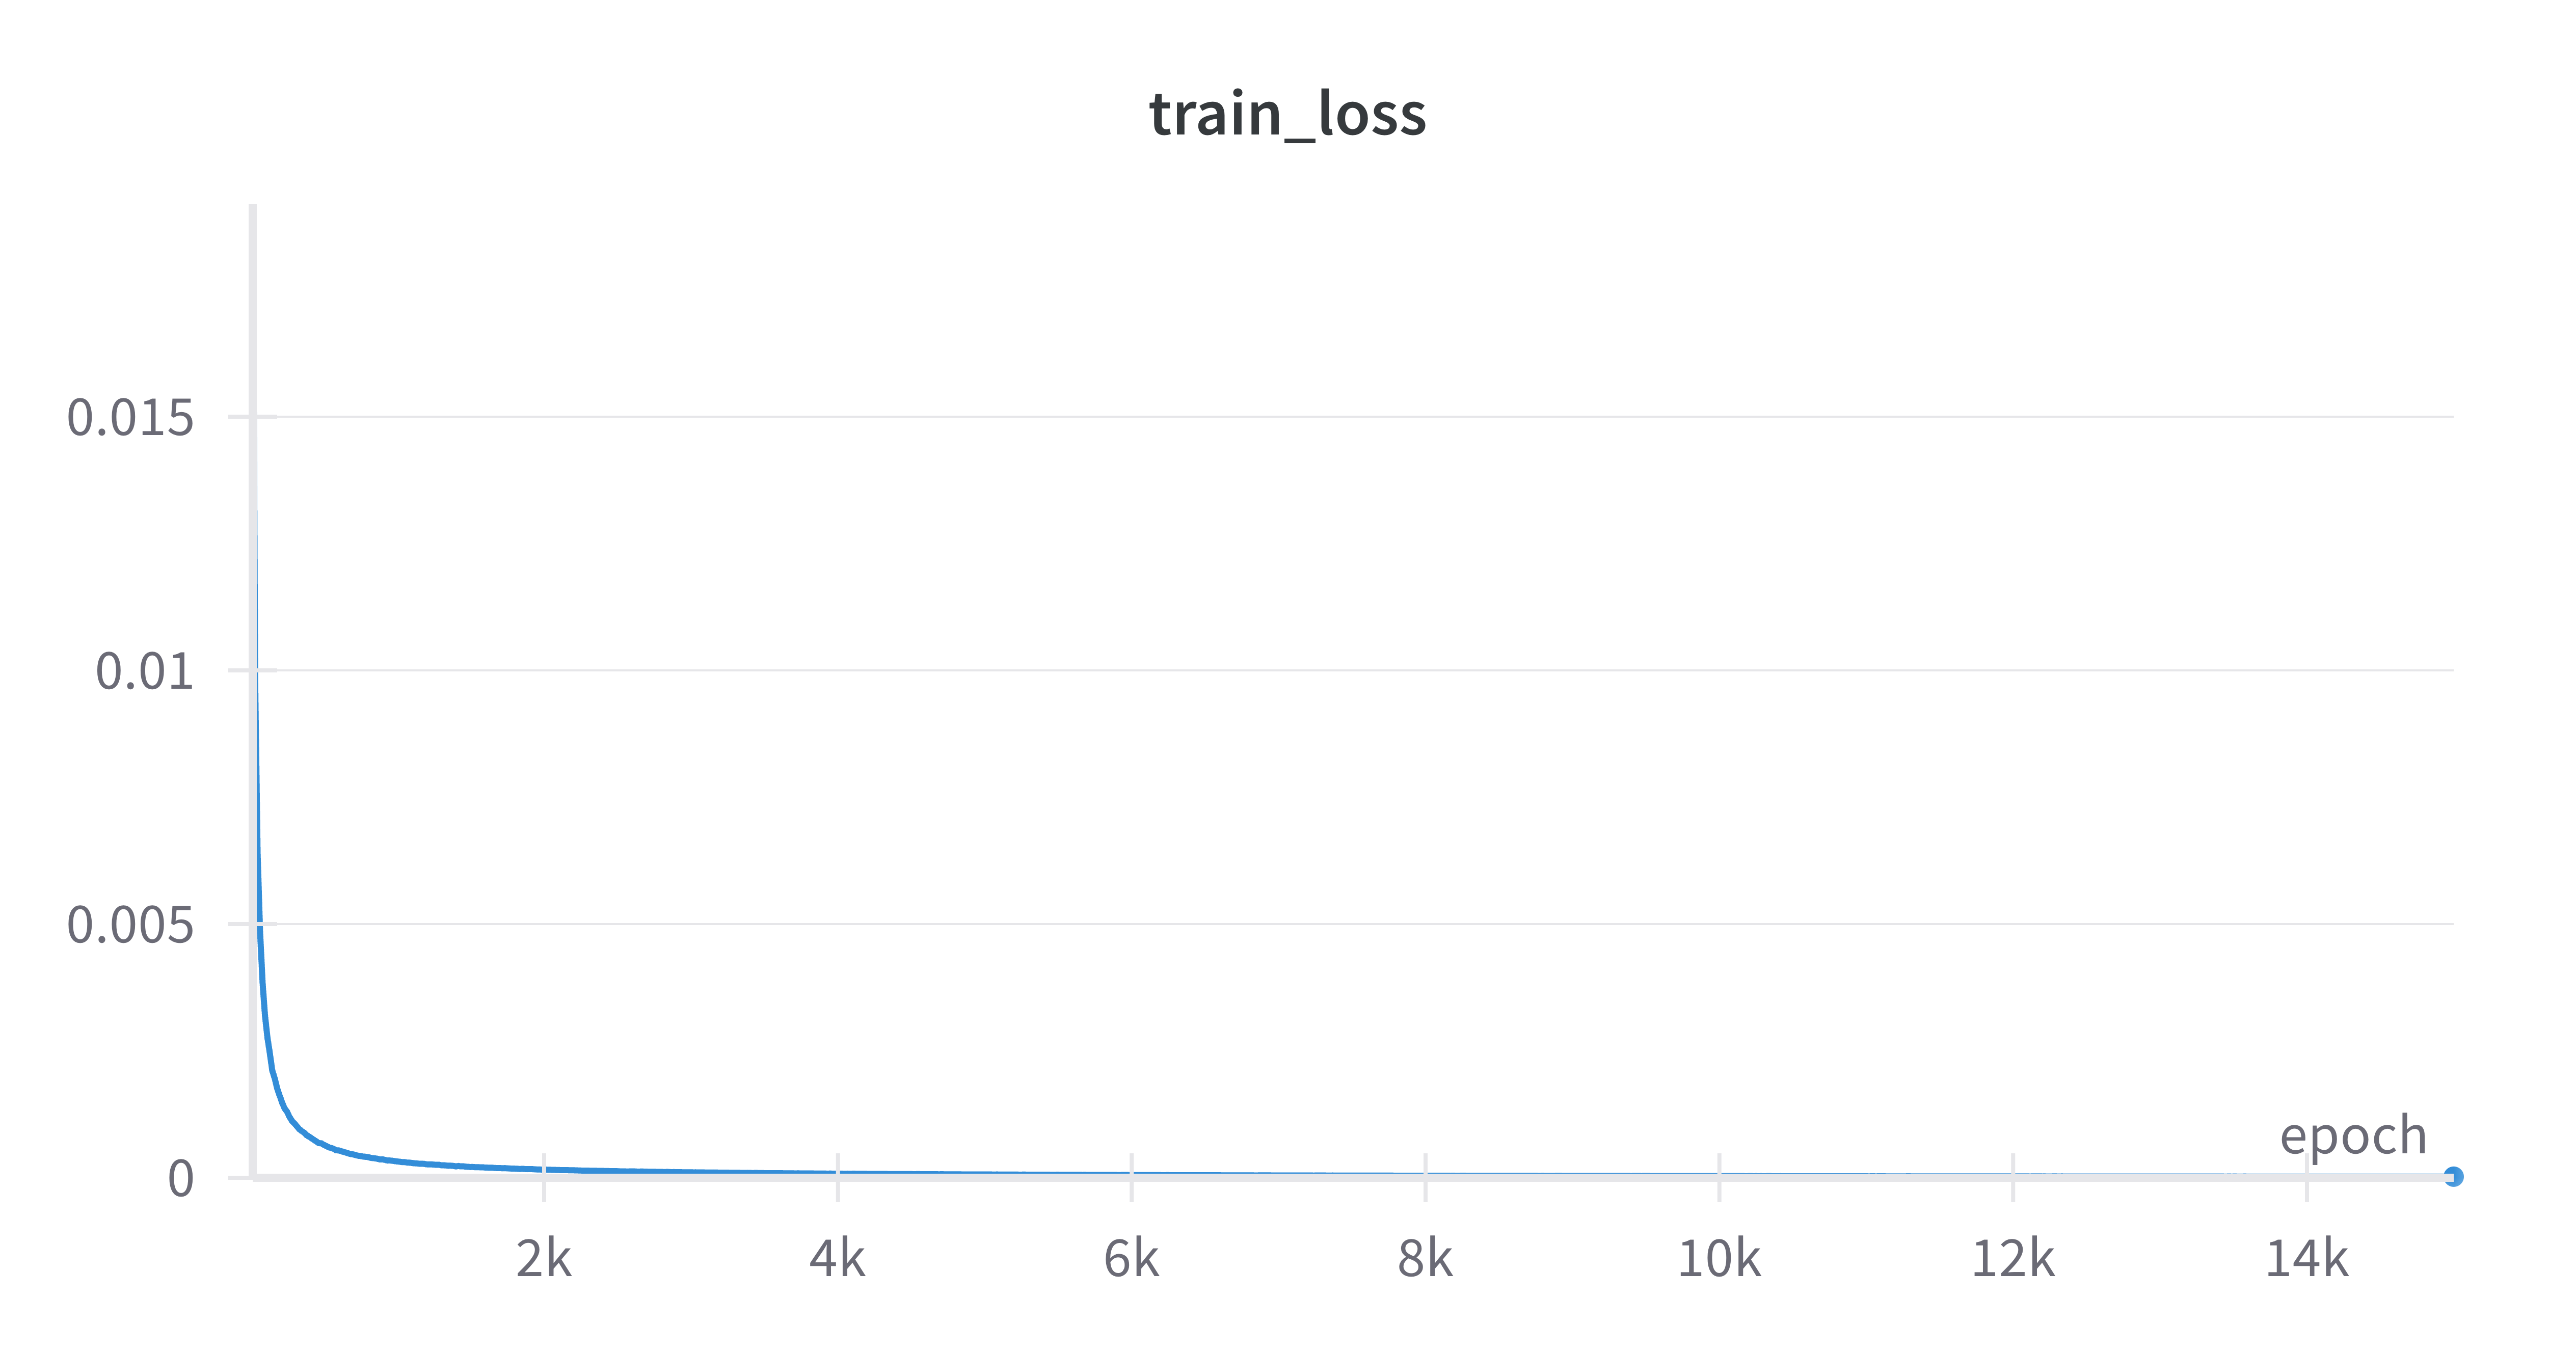
\includegraphics[width=\linewidth]{detailed_engineering/Monai Diffusion - Attempt 2/charts/train_loss.png}
\caption{}
\endminipage\hfill
\minipage{0.49\textwidth}
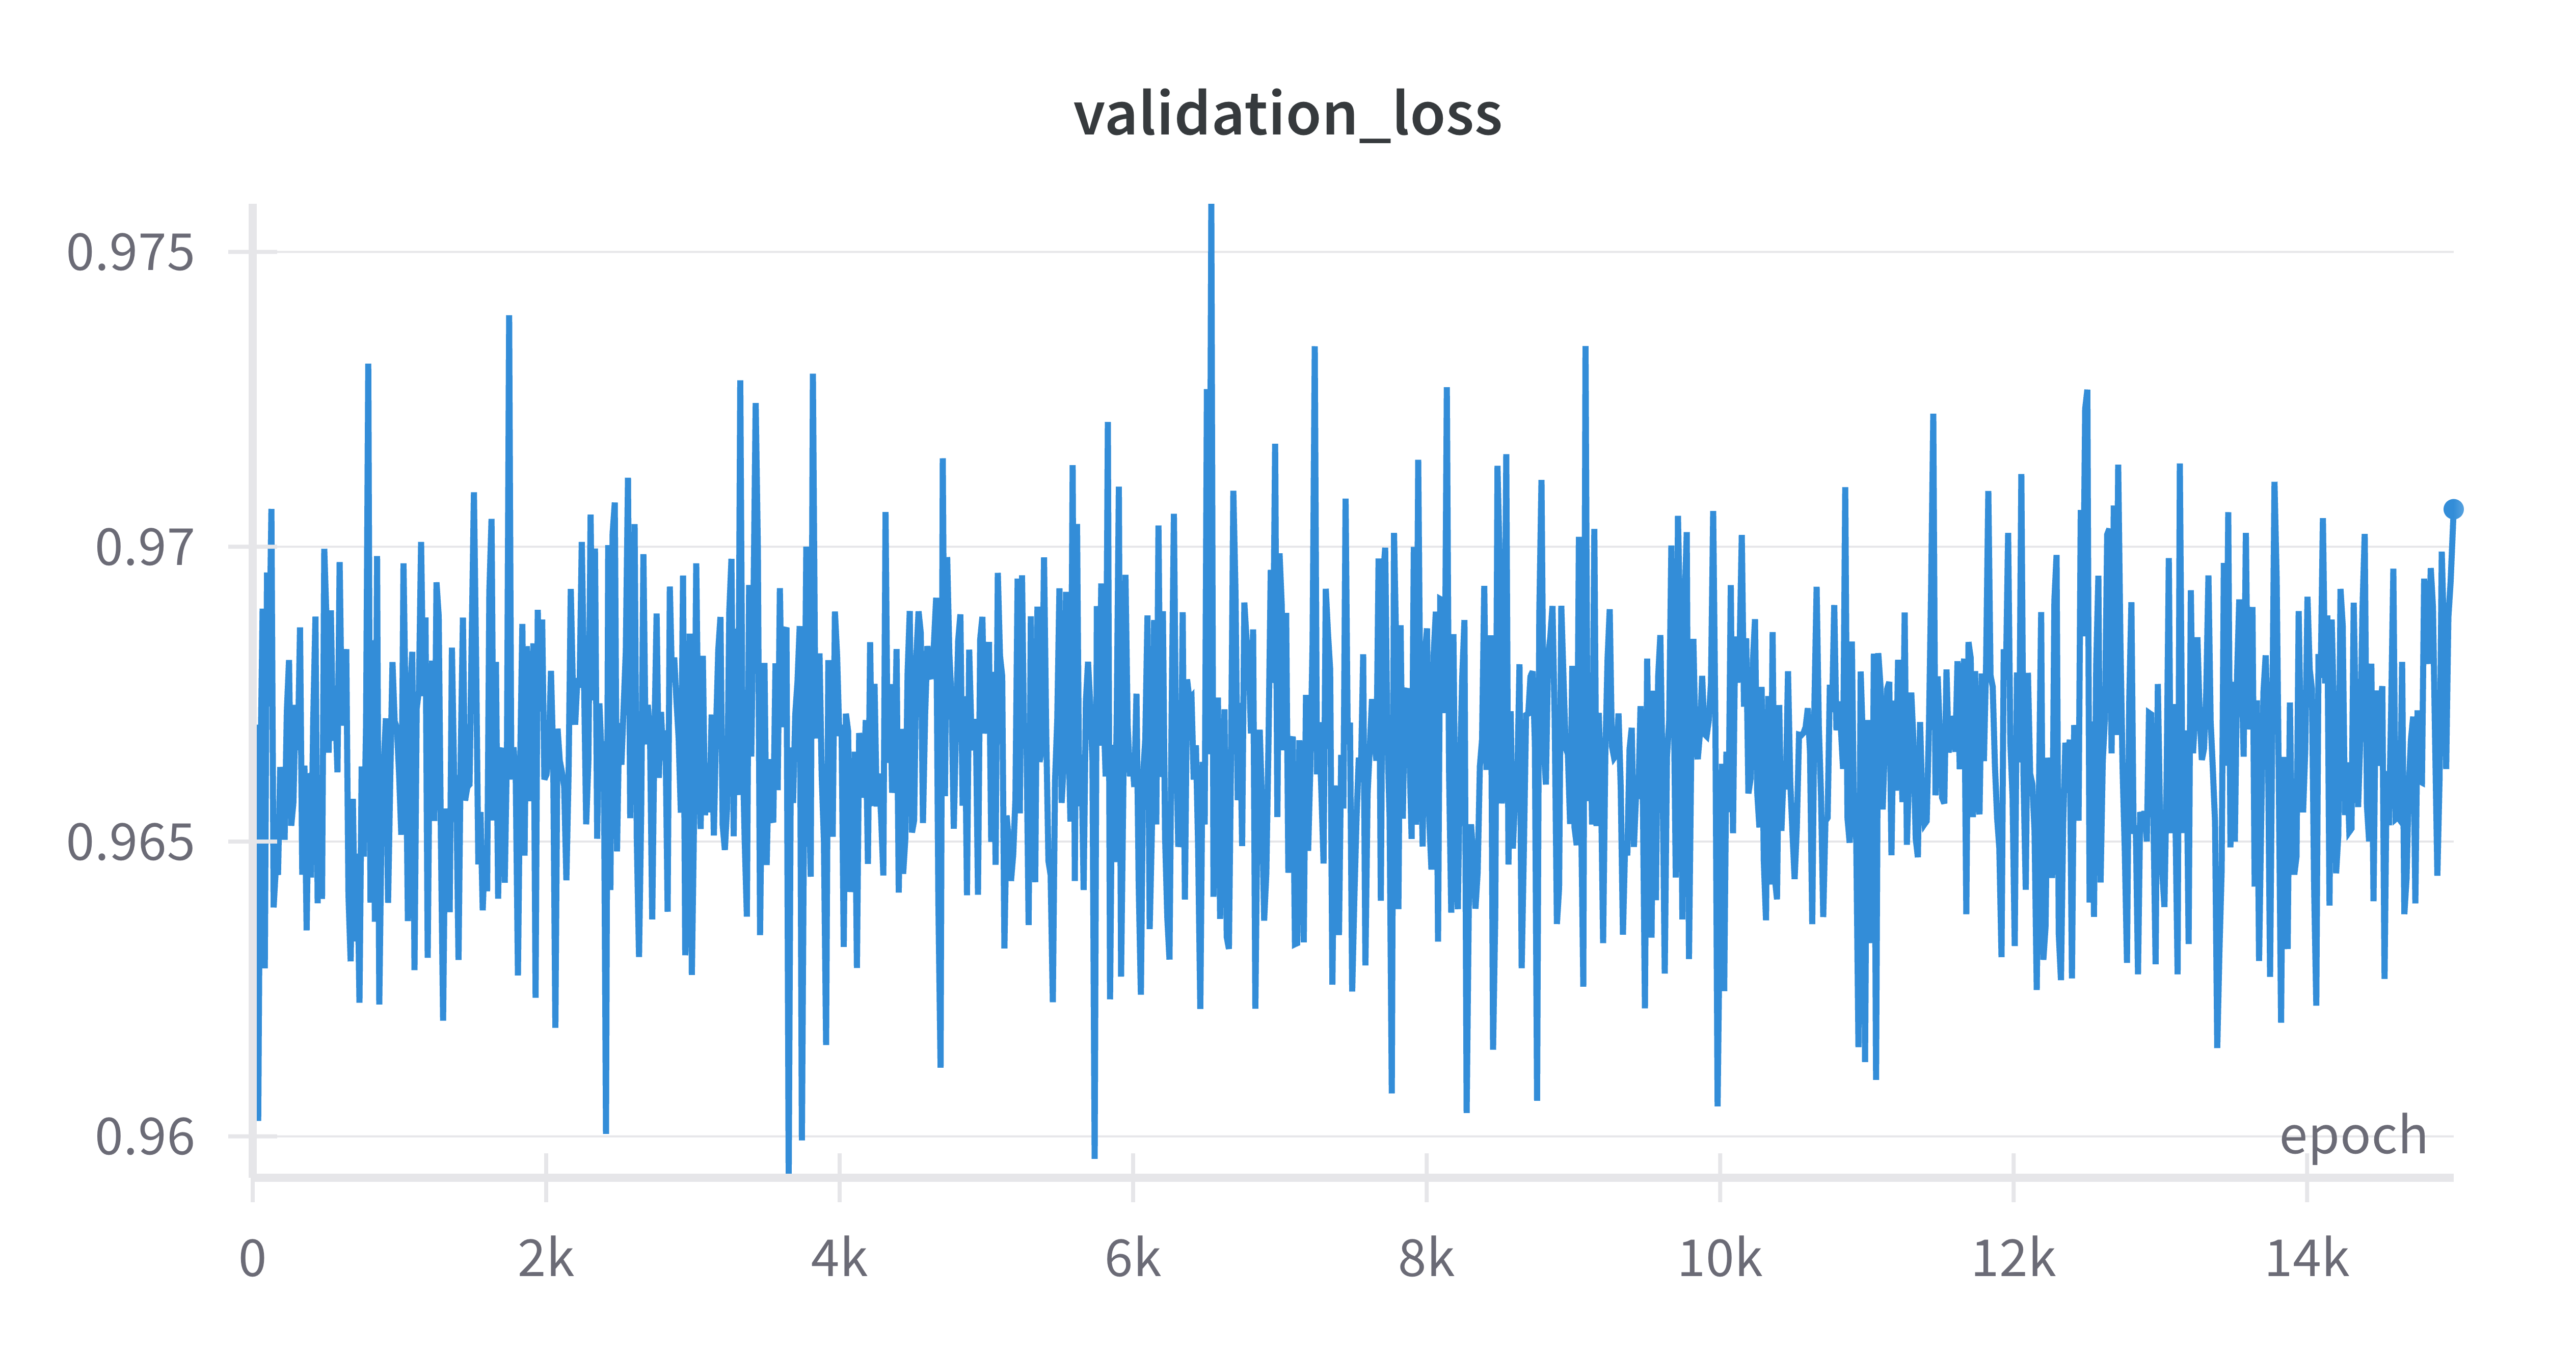
\includegraphics[width=\linewidth]{detailed_engineering/Monai Diffusion - Attempt 2/charts/validation_loss.png}
\caption{}
\label{fig:ldm_a2_val_loss}
\endminipage
\end{figure}

As is visible in the figure \ref{fig:ldm_a2_val_loss}, the validation loss did not decrease. The output of the generation was the same as in the previous attempt.


